\documentclass{article}
\usepackage[x11names, svgnames, rgb]{xcolor}
\usepackage[utf8]{inputenc}
\usepackage{tikz}
\usetikzlibrary{snakes,arrows,shapes}
\usepackage{amsmath}
\definecolor{lightcoral}{RGB}{240,128,128}
\definecolor{lightgreen}{RGB}{144,238,144}


%
%

%

%

\begin{document}
\pagestyle{empty}
%
%
%

\enlargethispage{100cm}
% Start of code
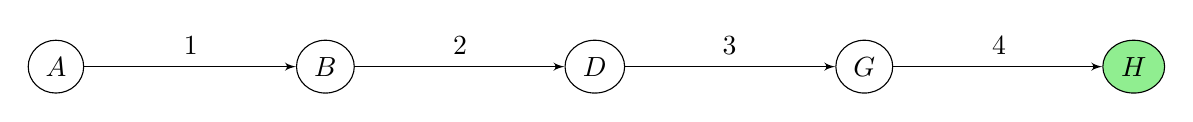
\begin{tikzpicture}[>=latex',line join=bevel,]
%%
\node (A) at (27.0bp,18.0bp) [draw,ellipse] {$A$};
  \node (B) at (124.0bp,18.0bp) [draw,ellipse] {$B$};
  \node (D) at (221.0bp,18.0bp) [draw,ellipse] {$D$};
  \node (G) at (318.0bp,18.0bp) [draw,ellipse] {$G$};
  \node (H) at (415.0bp,18.0bp) [draw,fill=lightgreen,ellipse] {$H$};
  \draw [->] (A) ..controls (64.13bp,18.0bp) and (75.802bp,18.0bp)  .. (B);
  \definecolor{strokecol}{rgb}{0.0,0.0,0.0};
  \pgfsetstrokecolor{strokecol}
  \draw (75.5bp,25.5bp) node {1};
  \draw [->] (B) ..controls (161.13bp,18.0bp) and (172.8bp,18.0bp)  .. (D);
  \draw (172.5bp,25.5bp) node {2};
  \draw [->] (D) ..controls (258.13bp,18.0bp) and (269.8bp,18.0bp)  .. (G);
  \draw (269.5bp,25.5bp) node {3};
  \draw [->] (G) ..controls (355.13bp,18.0bp) and (366.8bp,18.0bp)  .. (H);
  \draw (366.5bp,25.5bp) node {4};
%
\end{tikzpicture}
% End of code

%
\end{document}
%



